%!TEX program=xelatex+makeindex+bibtex
\documentclass[final]{scrreprt} %scrreprt of scrartcl
\input{../../library/preamble.tex}
\input{../../library/style.tex}
\addbibresource{../../library/bibliography.bib}

\begin{document}

\chapter{Labday 5: Localization using TDOA information}
\label{ch:labday5}
\section{Report 6}
\subsubsection{Basic localization}
We assumned before doing the TDOA estimation that the delay between sending and receiving in the audio buffer is known, ASIO provides a helpful function getLatencies for that, this function gives you the input and output delays in samples.
The delay time is mostly dependent on sampling frequency and buffer size.
When the full delays are known the calculation becomes a lot easier since it can be solved using two microphones only.
\\ \\
Figure \ref{fig:location} shows how the location of the car can be found when the locations of the microphones (and thus the distance between them, $a_1 + a_2$) and the time between transmission and arrivals at the two microphones $t_1$ and $t_2$, which can be converted into a distance using the speed of sound $c$ (Equation \ref{eq:speedofsound}).

\begin{equation}
c=\SI{343.2}{\meter\per\second}~\mathrm{for}~p = p_0~\mathrm{and}~T = \SI{293.15}{\kelvin}
\label{eq:speedofsound}
\end{equation}
Using this information, two possible locations can be found, the real location of the car and its mirrored version as shown in Figure \ref{fig:location}.

\begin{figure} [H]
\centering
	\begin{tikzpicture}	
		\node [anchor=east] at (0,0) (mic1) {Mic 1};
		\node [anchor=west] at (9,0) (mic2) {Mic 2};
		\node [anchor=south] at (6,3) (car) {Beacon};
		\node [anchor=north] at (4.5,-0.25) (a) {$a$};

		\draw (0,0) -- node[below]{$a_1$} (6,0)
			-- node[left]{$x$} (6,3)
			-- node[above, sloped]{$t_1 c$} (0,0);

		\draw (6,0) -- node[below]{$a_2$} (9,0)
			--  node[above, sloped]{$t_2 c$} (6,3);

		\draw [dotted] (0,0) -- (6,0)
			-- (6,-3)
			-- (0,0);

		\draw [dotted] (6,0) -- (9,0)
			--  (6,-3);
	\end{tikzpicture}
	\caption{Location determination.}
	\label{fig:location}
\end{figure}

From Figure \ref{fig:location}, equation \ref{eq:a1} and \label{eq:x} can be derived.
\begin{equation}
	a_1 = \frac{t_1^2 c^2 - t_2^2 c^2 + a^2}{2 a}
\label{eq:a1}
\end{equation}

\begin{equation}
	x = \sqrt{t_1^2 c^2 - a_1^2}
	\label{eq:x}
\end{equation}

To find the exact location of the beacon on the field when Mic 1 and Mic 2 are not on the same y-coordinate, an angular translation is needed as illustrated in Figure \ref{fig:angular-translation}.

\begin{figure} [H]
\centering
	\begin{tikzpicture}	
		\node [anchor=east] at (0,0) (mic1) {Mic 1};
		\node [anchor=south east] at (2.1213,6.3439) (car) {Beacon};
		\node [anchor=south west] at (1,0.15) {$\theta$};

		\draw [-*] (0,0) -- node[below]{$a_1$} (6,0)
			-- node[left]{$x$} (6,3);

		\draw [dashed, -*] (0,0) -- (4.2426,4.2426)
			-- (2.1213,6.3439);

		\draw [->] (1,0) arc (0:45:1);
	\end{tikzpicture}
	\caption{Angular translation.}
	\label{fig:angular-translation}
\end{figure}

\begin{equation}
	\theta = -\arctan{\frac{\text{Mic 2}_y - \text{Mic 1}_y}{\text{Mic 2}_x - \text{Mic 1}_x}}
	\label{eq:theta}
\end{equation}
Where $\theta$ is the angle between the two microphones.

The beacon location in x- and y-coordinates is found by adding the point ($a_1$, $x$) with an angular translation of $\theta$ to the location of Mic 1.
\\ \\
Since five microphones will be used instead of just two, the mirrored versions can be filtered out, leaving only the real location of the car as a solution.
By using only two microphones per location estimation instead of all five at once, wrong arrival times can be filtered out easily.
However, the arrival times are subject to errors, it might not be possible to filter the mirror images completely out of the solution sets.

\subsection{Height correction}
The height difference between the audio beacon and the microphones causes a larger time delay than expected when looking at the 2D plane.
However, this time delay can be corrected using Pythagoras' theorem (Equation \ref{eq:pythagoras}).

\begin{equation}
	t_{2D} = \sqrt{t_{3D}^2 - \Delta h^2}
	\label{eq:pythagoras}
\end{equation}

Where $\Delta h$ is the height difference between the beacon and the microphone.
The resulting $t_{2D}$ can be used in the basic localization to calculate the beacon location, independent of the height difference.

\subsection{TDOA to arrival times}
In order to use the TDOA data in the algorithm mentioned above, the time delays between the transmission and reception of the signal per microphone must be calculated from the TDOA data.
For this, it is known that this transition from TDOA to time delays is accomplished by adding a the same time constant time difference per microphone.
This constant is defined as the time difference between the absolute time of transmission and the absolute start time of the sample data, e.g. the absolute time of sample number one.
\\ \\
To find this constant, an orthogonal base of three microphones is used as in Figure \ref{fig:constant}.

\begin{figure} [H]
\centering
	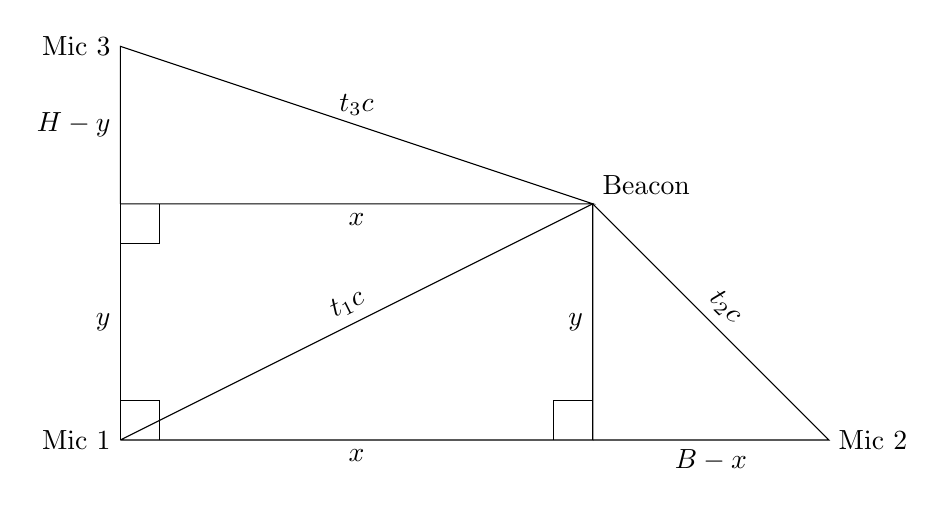
\begin{tikzpicture}	
		\node [anchor=east] at (0,0) (mic1) {Mic 1};
		\node [anchor=west] at (9,0) (mic2) {Mic 2};
		\node [anchor=east] at (0,5) (mic1) {Mic 3};
		\node [anchor=south west] at (6,3) (car) {Beacon};

		\draw (0,0) -- node[below]{$x$} (6,0)
			-- node[left]{$y$} (6,3)
			-- node[above, sloped]{$t_1 c$} (0,0);

		\draw (6,0) -- node[below]{$B - x$} (9,0)
			--  node[above, sloped]{$t_2 c$} (6,3);

		\draw (0,0) -- node[left]{$y$} (0,3);

		\draw (0,3) -- node[left]{$H - y$} (0,5)
			-- node[above]{$t_3 c$} (6,3)
			-- node[below]{$x$} (0,3);

		\draw (0.5,0) -- (0.5,0.5) -- (0,0.5);
		\draw (5.5,0) -- (5.5,0.5) -- (6,0.5);
		\draw (0,2.5) -- (0.5,2.5) -- (0.5,3);
	\end{tikzpicture}
	\caption{Model used for determination of the constant time error.}
	\label{fig:constant}
\end{figure}

Using the formula of the altitude of a triangle, e.g. $y$ in triangle (Mic 1, Mic 2, Beacon), the altitude is defined in equation \ref{eq:y1}.

\begin{equation}
	y = \frac{2 \sqrt{s(s - B)(s - D_1)(s - D_2)}}{B}
\label{eq:y1}
\end{equation}

With $B$ the base of the triangle, $D_1$ and $D_2$ the other two sides of the triangle and $s$ half of the perimeter of the triangle, $s = (B + D_1 + D_2) / 2$.
In the case of triangle (Mic 1, Mic 2, Beacon) with altitude line $y$, the base $B = \lVert Mic 1 - Mic 2 \rVert$ and the other two sides as $D_1 = t_1 c$ and $D_2 = t_2 c$ or vice versa.
\\ \\
For triangle (Mic 1, Mic 3, Beacon), $y$ is defined in equation \ref{eq:y2}.

\begin{equation}
	y = \frac{t_1^2 c^2 - t_3^2 c^2 + H^2}{2 B}
\label{eq:y2}
\end{equation}

The parameters $t_1$, $t_2$ and $t_3$ are defined with an offset of the constant we wish to find.
Using Equation \ref{eq:y1} and \ref{eq:y2}, which define the same $y$ since the three microphones form an orthogonal basis, and having an offset on $t_1$, $t_2$ and $t_3$, Matlab solved the formula of the constant using the script report6-2.m (Listing \ref{lst:report6-2.m}) from Appendix \ref{app:source}.
\\ \\
Now that the constant is known, the algorithm using two microphones and the arrival times can be applied.
It must be noted that the height difference between the microphones and the beacon is not considered in the calculation of the constant time offset.
Matlab could not find an explicit solution for the 3D situation, hence it was not included.
This will lead to an error in the resulting location.
However, the error will be very small when the beacon is not close to the microphone, hence only one microphone will be compromised at once.
For that, the base of orthogonal microphones shift to all four possible combinations and check for the best basis with the smallest standard deviation between the resulting locations, so the most tightly grouped solutions.
\\ \\
The final Matlab script can be found in Appendix \ref{app:source} Listing \ref{lst:location.m} location.m, which implements everything discussed so far in this chapter.

\subsection{Testing}
\label{sec:testing}
The test script location-errors.m as found in Appendix \ref{app:source} Listing \ref{lst:location.m} was used to find the error mean, standard deviation and maximum error.
The first test was in 2D mode; all microphones and the beacon were on the same height.
\\ \\
The other tests were with the four surrounding microphones 10 cm higher than the beacon and the last microphone 65 cm higher than the beacon.
The five microphones were set up as in the five microphone test setting from Labday 5.
All tests were done by calculating 2.500 points linearly spread on the 2.9m x 2.9m field.
The results are displayed in Table \ref{tab:errors}.

\begin{table} [H]
\centering
	\begin{tabular}{ c | c | c | c }
  	Setup & Error mean (mm) & Error standard deviation (mm) & Max error (mm) \\ \hline
  	2D & 0 & 0 & 0 \\
  	3D without height correction & 31.2 & 10.9 & 61.8 \\
	3D with height correction & 3.4 & 2.4 & 13.6 \\
	\end{tabular}
\caption{Location error details for different setups.}
\label{tab:errors}
\end{table}

\subsection{Testing with non-ideal data}
Errors will occur when the estimated speed of sound is not exactly correct since it varies with environment parameters such as temperature, humidity and air pressure (altitude).
Using the test script from the previous subsection \ref{sec:testing} with an altered speed of sound with the input data generation, a certain error will occur.
This was tested for the range of 1 to 5 percent deviation from the ``actual'' speed of sound, the results are shown in Table \ref{tab:c-errors}.

\begin{table} [H]
\centering
	\begin{tabular}{ c | c | c | c }
  	Deviation in speed of sound (\%) & Error mean (cm) & Error standard deviation (cm) & Max error (cm) \\ \hline
  	1 & 1.39 & 0.62 & 2.89 \\
	2 & 1.45 & 0.65 & 3.02 \\
	3 & 2.54 & 1.18 & 5.40 \\
	4 & 3.60 & 1.68 & 7.54 \\
  	5 & 3.12 & 1.09 & 6.18 \\
	\end{tabular}
\caption{Location error details for various deviations of the speed of sound.}
\label{tab:c-errors}
\end{table}

Besides errors in the speed of sound, errors can occur in determining the arrival times at the microphones.
These errors can be simulated using a normal distribution with varying standard deviations, the results are displayed in Table \ref{tab:std-errors}.
The noise standard deviation can be converted to standard deviation in distance by multiplying with the speed of sound.
At 0.15 ms, which corresponds to 5.1 cm, about 5 cm accuracy is achieved.

\begin{table} [H]
\centering
	\begin{tabular}{ c | c | c | c }
  	Noise standard deviation (ms) & Error mean (cm) & Error standard deviation (cm) & Max error (cm) \\ \hline
	0.1 & 3.34 & 1.88 & 11.88 \\
	0.15 & 4.90 & 2.97 & 50.51 \\
	0.2 & 6.70 & 5.00 & 125.76 \\
	0.3 & 11.34 & 9.02 & 127.42 \\
	0.4 & 16.35 & 13.55 & 180.23 \\
	0.5 & 23.03 & 21.88 & 292.76 \\
	\end{tabular}
\caption{Location error details for various arrival time error standard variations.}
\label{tab:std-errors}
\end{table}

\subsection{Testing with real measurement data}
The final test with five microphones, four in a 2.9m x 2.9m square on 38 cm height and one microphone placed 2.4 m from the center of the square on 0.93 cm high.
The car was placed on seven defined spots on the field, the first five at all microphones, the sixth at the center of the square and the last 1 m towards a corner of the square.
The recordings from the microphones were saved to be processed later on using the matched filter.
\\ \\
The matched filter however did not find the beacon signal accurately, which resulted in extremely bad results from the localization algorithm.
To get good input data for the localization algorithm anyway, a different Matlab script was used: Appendix A: process-mics.m.
This script looks for the first sample with amplitude of at least one third of the maximum sample amplitude for all inputted channels.
This sample number can be converted into a time value using the sample rate which can be directly inputted into the localization algorithm.
The results are shown in Figure \ref{fig:map}.
\\ \\
On this map all microphones and other test points are shown as dots and the calculated locations as crosses.
The five measurements at the microphones are not the exact places since the car could not come very close to the microphones, so the car was placed about 5 cm from the microphones toward the center of the room.
The microphone outside the square could not be localized, this is because the algorithm is made to work inside the square of microphones.
The algorithm fails when calculating the constant time offset, which becomes imaginary.
This will likely not be a problem since the car will stay inside the square in practice.
\\ \\
The error in the localization is less than 5 cm, also because the exact location of the car was not known since the car is rather large.
All together it can be concluded that the localization works with sufficient accuracy in practice too.

\begin{figure} [H]
\centering
	\begin{tikzpicture}	
		\fill[black,thick] (0, 0) circle [radius=0.5mm];
		\fill[black,thick] (0, 2.9*2) circle [radius=0.5mm];
		\fill[black,thick] (2.9*2, 2.9*2) circle [radius=0.5mm];
		\fill[black,thick] (2.9*2, 0) circle [radius=0.5mm];
		\fill[black,thick] (-1.05*2, 1.45*2) circle [radius=0.5mm];
		\fill[black,thick] (1.45*2, 1.45*2) circle [radius=0.5mm];
		\fill[black,thick] (1.45*2 + 0.707*2, 1.45*2 + 0.707*2) circle [radius=0.5mm];

		\draw (0.0014*2 + 0.1, 0.0810*2 + 0.1) -- (0.0014*2 - 0.1, 0.0810*2 - 0.1);
		\draw (0.0014*2 + 0.1, 0.0810*2 - 0.1) -- (0.0014*2 - 0.1, 0.0810*2 + 0.1);

		\draw (0.0435*2 + 0.1, 2.8779*2 + 0.1) -- (0.0435*2 - 0.1, 2.8779*2 - 0.1);
		\draw (0.0435*2 + 0.1, 2.8779*2 - 0.1) -- (0.0435*2 - 0.1, 2.8779*2 + 0.1);

		\draw (2.8450*2 + 0.1, 2.9414*2 + 0.1) -- (2.8450*2 - 0.1, 2.9414*2 - 0.1);
		\draw (2.8450*2 + 0.1, 2.9414*2 - 0.1) -- (2.8450*2 - 0.1, 2.9414*2 + 0.1);

		\draw (2.8536*2 + 0.1, 0.0276*2 + 0.1) -- (2.8536*2 - 0.1, 0.0276*2 - 0.1);
		\draw (2.8536*2 + 0.1, 0.0276*2 - 0.1) -- (2.8536*2 - 0.1, 0.0276*2 + 0.1);

		\draw (1.4312*2 + 0.1, 1.4258*2 + 0.1) -- (1.4312*2 - 0.1, 1.4258*2 - 0.1);
		\draw (1.4312*2 + 0.1, 1.4258*2 - 0.1) -- (1.4312*2 - 0.1, 1.4258*2 + 0.1);

		\draw (2.1686*2 + 0.1, 2.2024*2 + 0.1) -- (2.1686*2 - 0.1, 2.2024*2 - 0.1);
		\draw (2.1686*2 + 0.1, 2.2024*2 - 0.1) -- (2.1686*2 - 0.1, 2.2024*2 + 0.1);
	\end{tikzpicture}
	\caption{Map with errors.}
	\label{fig:map}
\end{figure}

\section{Porting to C\#}
Because we opted program the whole project in C\#, the algorithms made in the previous chapters needed to be ported to C\#. A rough test and LocationSystem library are included in Appendix Section \ref{appsec:ASIOTest} and \ref{appsec:LocationSystem}. The LocationSystem uses the ASIO driver interface, the obligatory inclusion of the copyright notice and logo not included in the software because it's not to be released.  Futer more we use the following libraries:
\begin{itemize}
\item BlueWave.Interop.Asio
\item CircularBuffer
\item MathNet.Numerics
\item Intel MKL
\item OxyPlot
\item OxyPlot.Wpf
\end{itemize}
All their dependencies are listed on the projects' websites.
\\ \\
\begin{figure}[h]
	\includegraphics[width=2cm]{resources/ASIO_LOGO1.jpg}
\end{figure}
ASIO Driver Interface Technology by Steinberg Media Technologies GmbH

\section{Conclusion}
The accuracy of the algorithm is sufficient, since the error mean and maximum are below $\SI{1}{\centi\meter}$ (Table \ref{tab:errors}).
A higher accuracy is not needed because other factors have a much bigger impact on the control of the car.

The height correction definitely adds accuracy to the location estimation as expected, hence it will be used later on.
This is however when the TDOA information is nearly infinitely accurate, which will not be the case.
The algorithm can give some erratic results when the measured time differences are erroneous.
To prevent these erratic results to disrupt the workings of the final system we will have to use for example a moving average filter for the position.
The car has a certain maximum distance it can move per time unit. We will use that knowledge to make sure the positions are not ``faulty'' of invalid.
\end{document}